Sesuai dengan daftar pengujian yang telah dilakukan pada subbab Pengujian \textit{Maintainability}, maka dapat dievaluasi sesuai dengan Tabel \ref{maintainability-evaluation}. Visualisasi perbandingan dapat dilihat lewat diagram garis pada Gambar \ref{diagram-pengguna-chart}. Dengan total skor 80\% yang tepat sama dengan \textit{evaluator goal} yang disebutkan pada subbab Deskripsi Pengujian \textit{Maintainability}, maka dapat dikatakan bahwa \textit{maintainability} pada sistem ini sudah cukup baik.

\LTXtable{\textwidth}{table/05/maintainability/recap_sorted}

\begin{figure}[h]
	\centering
	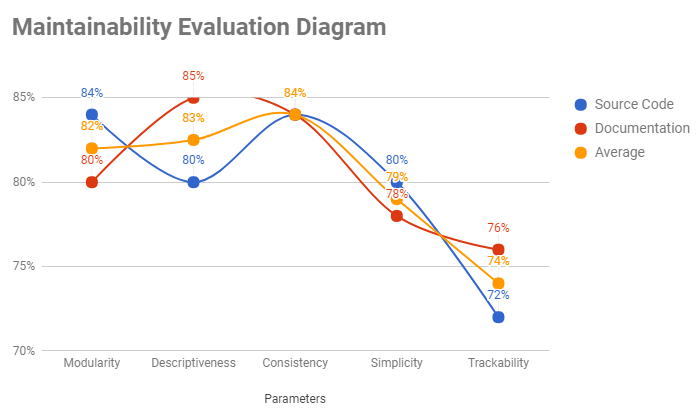
\includegraphics[width=\textwidth]{images/bab5/maintainability/maintainability-evaluation.png}
	\caption{Diagram Evaluasi Pengujian \textit{Maintainability}}
	\label{maintainability-diagram}
\end{figure}

\newpage